\documentclass[10pt]{article}
\usepackage[T1]{fontenc}
\usepackage[utf8]{inputenc}
\usepackage[english]{babel}
\usepackage{amsmath}
\usepackage{amssymb,mathrsfs}
\pagestyle{plain}
\usepackage{enumitem} 
\usepackage{amsthm}
\usepackage{titlesec}
\usepackage[all]{xy}
\usepackage[filecolor=green]{hyperref}
\usepackage{algorithm}
\usepackage{algorithmic}
\usepackage[toc,page]{appendix}
\usepackage{color}
\usepackage{listings}
\usepackage{xcolor}
\usepackage{multirow}
\usepackage{multicol}
\usepackage{tikz}
\usepackage{tikz-cd}

\newenvironment{changemargin}[2]{\begin{list}{}{%
      \setlength{\topsep}{0pt}%
      \setlength{\leftmargin}{0pt}%
      \setlength{\rightmargin}{0pt}%
      \setlength{\listparindent}{\parindent}%
      \setlength{\itemindent}{\parindent}%
      \setlength{\parsep}{0pt plus 1pt}%
      \addtolength{\leftmargin}{#1}%
      \addtolength{\rightmargin}{#2}%
    }\item }{\end{list}}


\newtheorem{theorem}{Theorem}
\newtheorem{proposition}{Proposition}
\newtheorem{corollary}{Corollary}
\newtheorem{lemma}{Lemma}


\usepackage[a4paper]{geometry}
\geometry{hscale=0.75,vscale=0.75,centering}
\bibliographystyle{plain}

\newcommand\N{\mathbb{N}}
\newcommand\g[1]{\textbf{#1}}
\newcommand\gth[1]{\emph{\g{#1}}}
\newcommand\id[1]{\text{id}_{#1}}
\newcommand\idd[1]{\emph{id}_{#1}}
\newcommand\zeroB[1]{0_{#1}}
\newcommand\unit[1]{1_{#1}}
\newcommand\im[1]{\text{im}\left(#1\right)}
\newcommand\sr[1]{\text{sr}\left(#1\right)}
\newcommand\one{\g{1}}
\newcommand\zero{\g{0}}
\newcommand\D{\g{D}}

\begin{document}

\section{Preliminaries}\label{sec:framework}

\paragraph{Notations.}

We fix the following notations:
\begin{itemize}
\item given a positive integer $n\in\N\setminus\{0\}$, we let
  $\overline{n}:=n-1$.
\item $e^n_i$ denotes the $i$-th vector of the canonical basis of the
  free module $\D^{1\times n}$.
\item We denote by $M^T$ the transpose matrix of $M$,
\item $p,\ p',\ q$ and $q'$ denote fixed integers, and we let $m:=p+p'$
  and $n:=q+p'+p+q'$.
\end{itemize}

\paragraph{Effective Fitting's Theorem.}

Let $\D$ be a ring, $R\in\D^{p\times q}$, $R\in\D^{p'\times q'}$
be two matrices and $\g{M}$ and $\g{M}'$ be the two left modules finitely
presented by $R$ and $R'$, respectively:
\begin{center}
  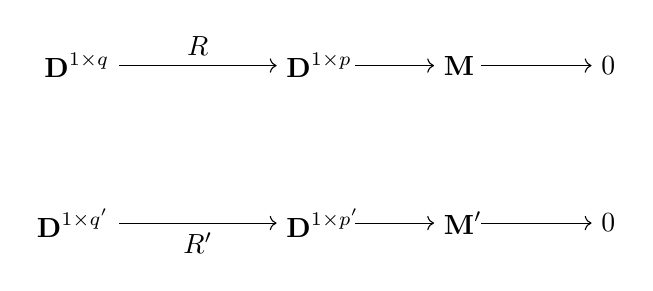
\begin{tikzpicture}
    \coordinate (Rel) at (-2, 0);
    \coordinate (Gen) at (0, 0);
    \coordinate (Genr) at (1, 0);
    \coordinate (M) at (2, 0);
    \coordinate (Mr) at (2.6, 0);
    \coordinate (Zero) at (4, 0);

    \coordinate (Relp) at (-2, -2);
    \coordinate (Genp) at (0, -2);
    \coordinate (Genpr) at (1, -2);
    \coordinate (Mp) at (2, -2);
    \coordinate (Mpr) at (2.6, -2);
    \coordinate (Zerop) at (4, -2);

    \coordinate (R) at (-1, 0);
    \coordinate (Rp) at (-1, -2);

    \draw[left] (Rel) node {$\D^{1\times q}$};
    \draw[right] (Gen) node {$\D^{1\times p}$};
    \draw[right] (M) node {$\g{M}$};
    \draw[right] (Zero) node {$0$};

    \draw[left] (Relp) node {$\D^{1\times q'}$};
    \draw[right] (Genp) node {$\D^{1\times p'}$};
    \draw[right] (Mp) node {$\g{M}'$};
    \draw[right] (Zerop) node {$0$};

    \draw[above] (R) node {$R$};
    \draw[below] (Rp) node {$R'$};
    
    \draw[->] (Rel) -- (Gen);
    \draw[->] (Genr) -- (M);
    \draw[->] (Mr) -- (Zero);
    
    \draw[->] (Relp) -- (Genp);
    \draw[->] (Genpr) -- (Mp);
    \draw[->] (Mpr) -- (Zerop);
    
  \end{tikzpicture}
\end{center}

Assume that there exists an isomorphism $\varphi:\g{M}\to\g{M}'$, so that
their exist matrices $P\in\D^{p\times p'}$, $P'\in\D^{p'\times p}$,
$Q\in\D^{q\times q'}$ and $Q'\in\D^{q'\times q}$ such that the
following diagram commutes:

\begin{center}
  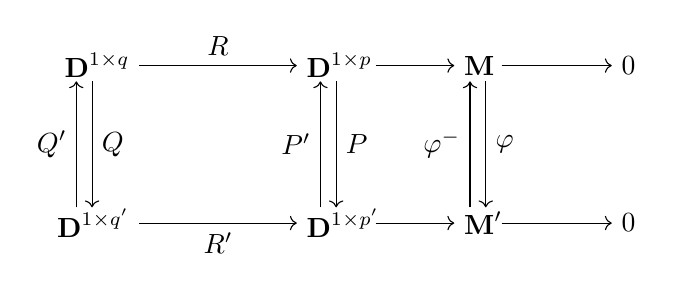
\begin{tikzpicture}
    \coordinate (Rel) at (-2, 0);
    \coordinate (Relsl) at (-2.8, -0.2);
    \coordinate (Relsr) at (-2.6, -0.2);
    \coordinate (Gen) at (0, 0);
    \coordinate (Genr) at (1, 0);
    \coordinate (Gensl) at (0.3, -0.2);
    \coordinate (Gensr) at (0.5, -0.2);
    \coordinate (M) at (2, 0);
    \coordinate (Mr) at (2.6, 0);
    \coordinate (Msl) at (2.2, -0.2);
    \coordinate (Msr) at (2.4, -0.2);
    \coordinate (Zero) at (4, 0);

    \coordinate (Relp) at (-2, -2);
    \coordinate (Relpnl) at (-2.8, -1.8);
    \coordinate (Relpnr) at (-2.6, -1.8);
    \coordinate (Genp) at (0, -2);
    \coordinate (Genpr) at (1, -2);
    \coordinate (Genpnl) at (0.3, -1.8);
    \coordinate (Genpnr) at (0.5, -1.8);
    \coordinate (Mp) at (2, -2);
    \coordinate (Mpr) at (2.6, -2);
    \coordinate (Mpnl) at (2.2, -1.8);
    \coordinate (Mpnr) at (2.4, -1.8);
    \coordinate (Zerop) at (4, -2);

    \coordinate (R) at (-1, 0);
    \coordinate (Rp) at (-1, -2);

    \coordinate (Qp) at (-2.8, -1);
    \coordinate (Q) at (-2.6, -1);

    \coordinate (Pp) at (0.3, -1);
    \coordinate (P) at (0.5, -1);

    \coordinate (phi) at (2.4, -1);
    \coordinate (phip) at (2.2, -1);

    \draw[left] (Rel) node {$\D^{1\times q}$};
    \draw[right] (Gen) node {$\D^{1\times p}$};
    \draw[right] (M) node {$\g{M}$};
    \draw[right] (Zero) node {$0$};

    \draw[left] (Relp) node {$\D^{1\times q'}$};
    \draw[right] (Genp) node {$\D^{1\times p'}$};
    \draw[right] (Mp) node {$\g{M}'$};
    \draw[right] (Zerop) node {$0$};

    \draw[above] (R) node {$R$};
    \draw[below] (Rp) node {$R'$};
    
    \draw[->] (Rel) -- (Gen);
    \draw[->] (Genr) -- (M);
    \draw[->] (Mr) -- (Zero);
    
    \draw[->] (Relp) -- (Genp);
    \draw[->] (Genpr) -- (Mp);
    \draw[->] (Mpr) -- (Zerop);

    \draw[->] (Mpnl) -- (Msl);
    \draw[->] (Msr) -- (Mpnr);

    \draw[->] (Genpnl) -- (Gensl);
    \draw[->] (Gensr) -- (Genpnr);

    \draw[->] (Relpnl) -- (Relsl);
    \draw[->] (Relsr) -- (Relpnr);

    \draw[left] (Qp) node {$Q'$};
    \draw[right] (Q) node {$Q$};

    \draw[left] (Pp) node {$P'$};
    \draw[right] (P) node {$P$};

    \draw[left] (phip) node {$\varphi^-$};
    \draw[right] (phi) node {$\varphi$};
  \end{tikzpicture}
\end{center}

Let us consider the two matrices
\[L:=\begin{pmatrix}
R & 0\\
0 & \id{p'}\\
0 & 0\\
0 & 0
\end{pmatrix},\ 
L':=\begin{pmatrix}
0 & 0\\
0 & 0\\
\id{p} & 0\\
0 & R'
\end{pmatrix}\in\D^{(q+p'+p+q')\times (p+p')}\]
Recall from~\cite{cluzeau2011constructive} that their exist matrices
$Z\in\D^{p\times q}$ $Z'\in\D^{p'\times q'}$, $R_2\in\D^{r\times q}$,
$R'_2\in\D^{r'\times q'}$, $Z_2\in\D^{q\times r}$ and $Z'_2\in\D^{q'
  \times r'}$
such that the following diagram commutes

\begin{center}
  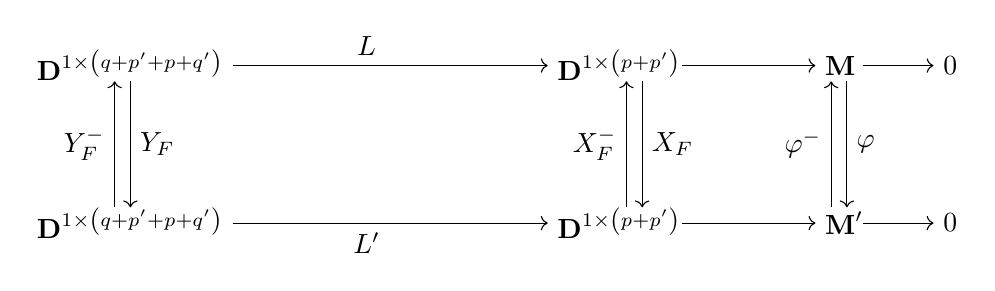
\begin{tikzpicture}
    \coordinate (Rel) at (-4, 0);
    \coordinate (Relsl) at (-5.5, -0.2);
    \coordinate (Relsr) at (-5.3, -0.2);
    \coordinate (Gen) at (0, 0);
    \coordinate (Genr) at (1.7, 0);
    \coordinate (Gensl) at (1, -0.2);
    \coordinate (Gensr) at (1.2, -0.2);
    \coordinate (M) at (3.4, 0);
    \coordinate (Mr) at (4, 0);
    \coordinate (Msl) at (3.6, -0.2);
    \coordinate (Msr) at (3.8, -0.2);
    \coordinate (Zero) at (4.9, 0);

    \coordinate (Relp) at (-4, -2);
    \coordinate (Relpnl) at (-5.5, -1.8);
    \coordinate (Relpnr) at (-5.3, -1.8);
    \coordinate (Genp) at (0, -2);
    \coordinate (Genpr) at (1.7, -2);
    \coordinate (Genpnl) at (1, -1.8);
    \coordinate (Genpnr) at (1.2, -1.8);
    \coordinate (Mp) at (3.4, -2);
    \coordinate (Mpr) at (4, -2);
    \coordinate (Mpnl) at (3.6, -1.8);
    \coordinate (Mpnr) at (3.8, -1.8);
    \coordinate (Zerop) at (4.9, -2);

    \coordinate (Rp) at (-2.3, -2);
    \coordinate (R) at (-2.3, 0);
    
    \coordinate (Qp) at (-5.5, -1);
    \coordinate (Q) at (-5.3, -1);

    \coordinate (Pp) at (1, -1);
    \coordinate (P) at (1.2, -1);

    \coordinate (phip) at (3.6, -1);
    \coordinate (phi) at (3.8, -1);
    
    \draw[left] (Rel) node {$\D^{1\times\left(q+p'+p+q'\right)}$};
    \draw[right] (Gen) node {$\D^{1\times\left(p+p'\right)}$};
    \draw[right] (M) node {$\g{M}$};
    \draw[right] (Zero) node {$0$};

    \draw[left] (Relp) node {$\D^{1\times\left(q+p'+p+q'\right)}$
    };
    \draw[right] (Genp) node {$\D^{1\times\left(p+p'\right)}$};
    \draw[right] (Mp) node {$\g{M}'$};
    \draw[right] (Zerop) node {$0$};

    \draw[above] (R) node {$L$};
    \draw[below] (Rp) node {$L'$};
    
    \draw[->] (Rel) -- (Gen);
    \draw[->] (Genr) -- (M);
    \draw[->] (Mr) -- (Zero);
    
    \draw[->] (Relp) -- (Genp);
    \draw[->] (Genpr) -- (Mp);
    \draw[->] (Mpr) -- (Zerop);

    \draw[->] (Mpnl) -- (Msl);
    \draw[->] (Msr) -- (Mpnr);

    \draw[->] (Genpnl) -- (Gensl);
    \draw[->] (Gensr) -- (Genpnr);

    \draw[->] (Relpnl) -- (Relsl);
    \draw[->] (Relsr) -- (Relpnr);

    \draw[left] (Qp) node {$Y_{F}^-$};
    \draw[right] (Q) node {$Y_{F}$};

    \draw[left] (Pp) node {$X_{F}^-$};
    \draw[right] (P) node {$X_{F}$};

    \draw[left] (phip) node {$\varphi^-$};
    \draw[right] (phi) node {$\varphi$};
  \end{tikzpicture}
\end{center}
where
\[\begin{split}
X_F&:=\begin{pmatrix}
\id{p} & P\\
-P' & \id{p'}-P'P
\end{pmatrix},\ \
Y_F:=\begin{pmatrix}
\id{q} & 0 & R & Q\\
0 & \id{p'} & -P' & Z'\\
-Z & P & 0 & PZ'-ZQ\\
-Q' & -R' & 0 & Z'_2R'_2
\end{pmatrix}\\
& \\
X_F^-&:=\begin{pmatrix}
\id{p}-PP' & -P\\
P' & \id{p'}
\end{pmatrix},\ \
Y_F^-:=\begin{pmatrix}
Z_2R_2 & 0 & -R & -Q\\
P'Z-Z'Q' & 0 & P' & -Z'\\
Z & -P & \id{p} & 0\\
Q' & R' & 0 & \id{q'}
\end{pmatrix}.\\
\end{split}\]

\section{Reduction of the zero bloc}

Assume that $q+p'\leq p+q'$ and $\sr{\D}\leq\overline{p+q'}$. We let
\[\tilde{L}:=\begin{pmatrix}
R & 0\\
0 & \id{p'}\\
0 & 0\\
0 & 0
\end{pmatrix}\in\D^{\overline{n}\times m}\ \
\text{and}\ \
\tilde{L}':=\begin{pmatrix}
0 & 0\\
0 & 0\\
\id{p} & 0\\
0 & R'
\end{pmatrix}\in\D^{\overline{n}\times m}.\]

\begin{proposition}\label{prop:reduced_Bezout_zero_part}
  There exist lines $\gth{c},\ \gth{u}\in\gth{D}^{1\times p}$ and
  $\gth{d},\ \gth{v}\in\gth{D}^{1\times\overline{q'}}$ such that
  \begin{equation}\label{equ:reduced_Bezout_zero_part}
    \begin{pmatrix}
      0 & \gth{c} & \gth{d}\end{pmatrix}\begin{pmatrix}
      \idd{q+p'} & 0 & 0 & 0\\
      0 & \idd{p} & 0 & \gth{u}^T\\
      0 & 0 & \idd{\overline{q'}} & \gth{v}^T
    \end{pmatrix}Y_F(e^{n}_{q+p'})^T=1.
  \end{equation}

\end{proposition}

\begin{proof}
  Getting terms of the $p'$-th column and $p'$-th line in the relation
  $\id{p'}=P'P+Z'R'$, we get the following:
  \[\sum_{k=1}^pP'_{p'k}P_{kp'}+\sum_{k=1}^{q'}Z'_{p'k}R'_{kp'}=1.\]
  From $\sr{\D}\leq\overline{p+q'}$, we deduce that there exist $c_1,
  \cdots,\ c_p,\ d_1,\cdots,\ d_{\overline{q'}},\ u_1,\cdots,\ u_p,\ v_1,
  \cdots,\ v_{\overline{q'}}\in\D$ such that
  \begin{equation}\label{equ:reduced_Bezout_zero_part_proof}
    \sum_{k=1}^pc_k\left(P_{kp'}+u_kR'_{q'p'}\right)+\sum_{k=1}^{
      \overline{q'}}d_k\left(R'_{kp'}+v_kR'_{q'p'}\right)=1.
  \end{equation}
  Letting $\g{c}:=\left(c_1,\cdots,\ c_p\right)$, $\g{d}:=\left(-d_1,
  \cdots,\ -d_{\overline{q'}}\right)$, $\g{u}:=\left(-u_1,\cdots,\ -u_p
  \right)$ and $\g{v}:=\left(v_1,\cdots,\ v_{\overline{q'}}\right)$, the
  hand side of \eqref{equ:reduced_Bezout_zero_part_proof} is the left
  hand side of \eqref{equ:reduced_Bezout_zero_part}, which proves
  Proposition~\ref{prop:reduced_Bezout_zero_part}.
\end{proof}

With the notations of Proposition~\ref{prop:reduced_Bezout_zero_part},
we introduce the lines $\tilde{\ell}\in\D^{1\times\overline{n}}$ and $
\ell\in\D^{1\times n}$ defined as follows:
\[\tilde{\ell}:=\begin{pmatrix}
0 & \g{c} & \g{d}\end{pmatrix}\ \ \text{and}\ \
\ell:=\begin{pmatrix}
0 & \g{c} & \g{d} & 0
\end{pmatrix},\]
as well as the matrices $U\in\D^{n\times n}$, $F\in\D^{\overline{n}\times
  n}$ defined as follows:
\[U:=\begin{pmatrix}
\id{q+p'} & 0 & 0 & 0\\
0 & \id{p} & 0 & \g{u}^T\\
0 & 0 & \id{\overline{q'}} & \g{v}^T\\
0 & 0 & 0 & 1
\end{pmatrix}\ \ \text{and}\ \
F:=\begin{pmatrix}
\id{\overline{n}} & 0
\end{pmatrix}UY_F.\]

\begin{corollary}\label{cor:extended_Bezout_zero_part}
  We have:
  \begin{equation}\label{equ:extend_Bezout_zero_part}
    1=\tilde{\ell}F(e^n_{q+p'})^T=\ell UY_F(e^n_{q+p'})^T,
  \end{equation}
\end{corollary}

\begin{proof}
  The first equality is a consequence of Relation
  \eqref{equ:reduced_Bezout_zero_part} and the following relation:
  \[F=\begin{pmatrix}
  \id{q+p'} & 0 & 0 & 0\\
  0 & \id{p} & 0 & \g{u}^T\\
  0 & 0 & \id{\overline{q'}} & \g{v}^T
  \end{pmatrix}Y_F.
  \]
  The second equality is due to the definitions of $\tilde{\ell}$, $\ell$
  and $F$.
\end{proof}

We consider the matrices $\pi,\ \pi'\in\D^{n\times\overline{n}}$ and
$\iota,\ \iota'\in\D^{\overline{n}\times n}$ defined as follows:
\[\begin{tabular}{l l}
$\pi:=\begin{pmatrix}
\id{\overline{n}}-F(e^{n}_{q+p'})^T\tilde{\ell}\\
\tilde{\ell}
\end{pmatrix}$,
&
$\pi':=\left(\id{n}-(e^{n}_{q+p'})^T\ell UY_F\right)\begin{pmatrix}
  \id{q+\overline{p'}} & 0\\
  0 & 0\\
  0 & \id{p+q'}
\end{pmatrix}$,
\\
&
\\
$\iota:=\begin{pmatrix}
\id{\overline{n}}-F(e^{n}_{q+p'})^T\tilde{\ell} &
F(e^{n}_{q+p'})^T
\end{pmatrix}$,
&
$\iota':=\begin{pmatrix}
\id{q+\overline{p'}} & 0 & 0\\
0 & 0 & \id{p+q'}
\end{pmatrix}$.
\end{tabular}\]

\begin{proposition}\label{prop:exact_sequences_zero_part}
  We have the following relations
  \begin{multicols}{2}
    \begin{enumerate}
    \item\label{it:split_pi_zero_part} $\iota\pi=\idd{\overline{n}}$,
    \item\label{it:split_pip_zero_part} $\iota'\pi'=\idd{\overline{n}}$,
    \item\label{it:ker_pi_zero_part} $\ker(.\pi)=\emph{\D}\ell$,
    \item\label{it:ker_pip_zero_part} $\ker(.\pi')=\emph{\D}\ell UY_F$.
    \end{enumerate}
  \end{multicols}
\end{proposition}

\begin{proof}
  \begin{enumerate}
  \item From \eqref{equ:extend_Bezout_zero_part}, we have $\left(F(
    e^{n}_{q+p'})^T\tilde{\ell}\right)^2=F(e^{n}_{q+p'})^T\tilde{\ell}$,
    from which we deduce $\iota\pi=\id{\overline{n}}$ by computing the
    matrix product. 
  \item We have $\iota'(e^n_{q+p'})^T=0$, from which we deduce $\iota'
    \pi'=\id{\overline{n}}$ by computing the matrix product.
  \item By considering the natural isomorphism $\D^{1\times n}\simeq
    \D^{1\times\overline{n}}\oplus\D$, we have $\pi=\pi_1\pi_2$,
    where $\pi_1\in\D^{n\times n}$ and $\pi_2\in\D^{n\times \overline{n}}$
    are defined as follows:
    \[\pi_1:=\begin{pmatrix}
    \id{\overline{n}}-F(e^{n}_{q+p'})^T\tilde{\ell} & 0\\
    0 & 1
    \end{pmatrix}\ \ \text{and}\ \
    \pi_2:=\begin{pmatrix}
    \id{\overline{n}}\\
    \tilde{\ell}
    \end{pmatrix}.\]
    From \eqref{equ:extend_Bezout_zero_part}, $\im{.\pi_1}$ is included in
    $\ker(.F(e^{n}_{q+p'})^T)\oplus\D$ and the restriction of $.\pi_2$ to
    the latter is injective: for $(u,x)\in\left(\ker(.F(e^{n}_{q+p'})^T)
    \oplus\D\right)\cap\ker(.\pi_2)$, we have $u+x\tilde{\ell}=0$, which
    gives $x=0$ and $u=0$ by \eqref{equ:extend_Bezout_zero_part}. Hence, we
    have $\ker(.\pi)=\ker(.\pi_1)=\ker\left(\id{\overline{n}}-.F(e^{n}_{q+
      p'})^T\tilde{\ell}\right)\oplus 0$. We conclude by showing $\ker
    \left(\id{\overline{n}}- .F(e^{n}_{q+p'})^T\tilde{\ell}\right)=\D
    \tilde{\ell}$: the right to left inclusion is due to
    \eqref{equ:extend_Bezout_zero_part}, and the other one is due to the
    relation $x=\left(xF(e^n_{q+p'})^T\right)\tilde{\ell}$, for every $x\in
    \ker\left(\id{\overline{n}}-.F(e^n_{q+p'})^T\tilde{\ell}\right)$.
  \item From \eqref{equ:extend_Bezout_zero_part}, we have 
    $\D\ell UY_F\subseteq\ker(.\pi')$. The converse inclusion is due to the
    relation $x=x_{q+p'}\ell UY_F$, for every $x\in\ker(.\pi')$. Indeed,
    the first $q+\overline{p'}$ and the last $p+q'$ columns of $x$ and
    $x_{q+p'}\ell UY_F$ are equal since $x\in\ker(.\pi')$ implies
    \begin{equation}\label{equ:ker_pip_zero_part_1}
      x\begin{pmatrix}
      \id{q+\overline{p'}} & 0\\
      0 & 0\\
      0 & \id{p+q'}
      \end{pmatrix}=x_{q+p'}\ell UY_F\begin{pmatrix}
      \id{q+\overline{p'}} & 0\\
      0 & 0\\
      0 & \id{p+q'}
      \end{pmatrix}.
    \end{equation}
    Moreover, the $q+p'$-th colums of $x_{q+p'}\ell UY_F$ is computed
    by right multiplication by $(e^n_{q+p'})^T$ and is equal to
    $x_{q+p'}$ from \eqref{equ:extend_Bezout_zero_part}.
  \end{enumerate}
\end{proof}

\begin{theorem}\label{thm:reduction_id}
  With the previous notations, we let
  \[Y_W:=\iota UY_F\pi'\ \ \text{and}\ \ Y_W^-:=\iota'Y_F^-U^-\pi.\]
  The following diagram is exact and commutative:
  \begin{center}
    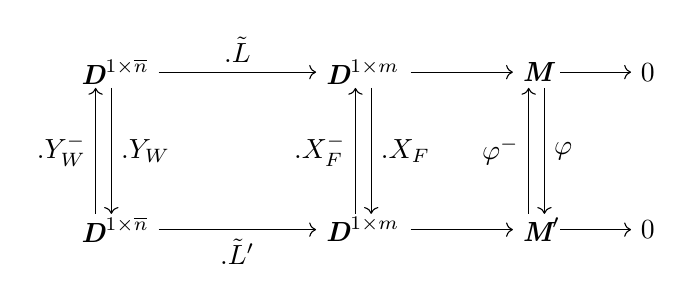
\begin{tikzpicture}
      \coordinate (Rel) at (-4, 0);
      \coordinate (Relsl) at (-4.8, -0.2);
      \coordinate (Relsr) at (-4.6, -0.2);
      \coordinate (Gen) at (-2, 0);
      \coordinate (Genr) at (-0.8, 0);
      \coordinate (Gensl) at (-1.5, -0.2);
      \coordinate (Gensr) at (-1.3, -0.2);
      \coordinate (M) at (0.5, 0);
      \coordinate (Mr) at (1.1, 0);
      \coordinate (Msl) at (0.7, -0.2);
      \coordinate (Msr) at (0.9, -0.2);
      \coordinate (Zero) at (2, 0);

      \coordinate (Relp) at (-4, -2);
      \coordinate (Relpnl) at (-4.8, -1.8);
      \coordinate (Relpnr) at (-4.6, -1.8);
      \coordinate (Genp) at (-2, -2);
      \coordinate (Genpr) at (-0.8, -2);
      \coordinate (Genpnl) at (-1.5, -1.8);
      \coordinate (Genpnr) at (-1.3, -1.8);
      \coordinate (Mp) at (0.5, -2);
      \coordinate (Mpr) at (1.1, -2);
      \coordinate (Mpnl) at (0.7, -1.8);
      \coordinate (Mpnr) at (0.9, -1.8);
      \coordinate (Zerop) at (2, -2);

      \coordinate (R) at (-3, 0);
      \coordinate (Rp) at (-3, -2);

      \coordinate (Qp) at (-4.8, -1);
      \coordinate (Q) at (-4.6, -1);

      \coordinate (Pp) at (-1.5, -1);
      \coordinate (P) at (-1.3, -1);

      \coordinate (phi) at (0.9, -1);
      \coordinate (phip) at (0.7, -1);

      \draw[left] (Rel) node {$\emph{\D}^{1\times\overline{n}}$};
      \draw[right] (Gen) node {$\emph{\D}^{1\times m}$};
      \draw[right] (M) node {$\emph{\g{M}}$};
      \draw[right] (Zero) node {$0$};

      \draw[left] (Relp) node {$\emph{\D}^{1\times\overline{n}}$
      };
      \draw[right] (Genp) node {$\emph{\D}^{1\times m}$};
      \draw[right] (Mp) node {$\emph{\g{M}}'$};
      \draw[right] (Zerop) node {$0$};

      \draw[above] (R) node {$.\tilde{L}$};
      \draw[below] (Rp) node {$.\tilde{L}'$};
      
      \draw[->] (Rel) -- (Gen);
      \draw[->] (Genr) -- (M);
      \draw[->] (Mr) -- (Zero);
      
      \draw[->] (Relp) -- (Genp);
      \draw[->] (Genpr) -- (Mp);
      \draw[->] (Mpr) -- (Zerop);

      \draw[->] (Mpnl) -- (Msl);
      \draw[->] (Msr) -- (Mpnr);

      \draw[->] (Genpnl) -- (Gensl);
      \draw[->] (Gensr) -- (Genpnr);

      \draw[->] (Relpnl) -- (Relsl);
      \draw[->] (Relsr) -- (Relpnr);

      \draw[left] (Qp) node {$.Y_{W}^-$};
      \draw[right] (Q) node {$.Y_{W}$};

      \draw[left] (Pp) node {$.X_{F}^-$};
      \draw[right] (P) node {$.X_{F}$};

      \draw[left] (phip) node {$\varphi^-$};
      \draw[right] (phi) node {$\varphi$};
    \end{tikzpicture}

  \end{center}
\end{theorem}

\begin{proof}
  We only have to show that the diagram is commutative.
  
  First, we show that $Y_W$ and $Y_W^-$ are inverse to each other.
  From Proposition~\ref{prop:exact_sequences_zero_part}, the lines of the
  following diagram are exact
  \begin{center}
    \begin{equation}\label{equ:diagram_reduction_zero}
      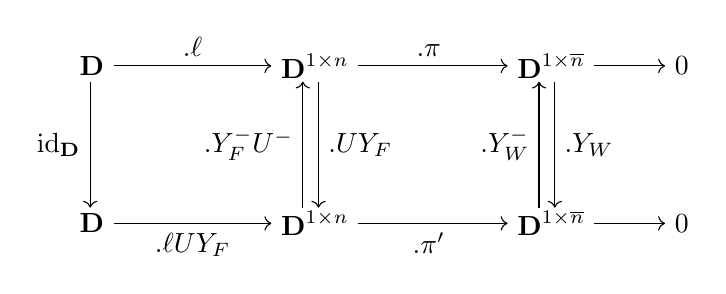
\begin{tikzpicture}
        \coordinate (Rel) at (-2,0);
        \coordinate (Rels) at (-2.3, -0.2);
        \coordinate (Gen) at (0, 0);
        \coordinate (Gensl) at (0.4, -0.2);
        \coordinate (Gensr) at (0.6, -0.2);
        \coordinate (Genr) at (1.1, 0);
        \coordinate (M) at (3, 0);
        \coordinate (Msl) at (3.4, -0.2);
        \coordinate (Msr) at (3.6, -0.2);
        \coordinate (Mr) at (4.1, 0);
        \coordinate (zero) at (5, 0);

        \coordinate (R) at (-1, 0);
        \coordinate (pi) at (2, 0);

        \coordinate (Relp) at (-2,-2);
        \coordinate (Relpn) at (-2.3, -1.8);
        \coordinate (Genp) at (0, -2);
        \coordinate (Genpnl) at (0.4, -1.8);
        \coordinate (Genpnr) at (0.6, -1.8);
        \coordinate (Genrp) at (1.1, -2);
        \coordinate (Mp) at (3, -2);
        \coordinate (Mpnl) at (3.4, -1.8);
        \coordinate (Mpnr) at (3.6, -1.8);
        \coordinate (Mpr) at (4.1, -2);
        \coordinate (zerop) at (5, -2);

        \coordinate (Rp) at (-1, -2);
        \coordinate (pip) at (2, -2);

        
        \coordinate (Q) at (-2.3, -1);
        \coordinate (P) at (0.6, -1);
        \coordinate (Pp) at (0.4, -1);
        \coordinate (phi) at (3.6, -1);
        \coordinate (phip) at (3.4, -1);

        \draw[left] (Q) node {$\id{\D}$};
        \draw[left] (Pp) node {$.Y_F^-U^-$};
        \draw[right] (P) node {$.UY_F$};
        \draw[left] (phip) node {$.Y_W^-$};
        \draw[right] (phi) node {$.Y_W$};
        
        
        \draw[left] (Rel) node {$\D$};
        \draw[right] (Gen) node {$\D^{1\times n}$};
        \draw[right] (M) node {$\D^{1\times \overline{n}}
          $};
        \draw[right] (zero) node {$0$};

        \draw[above] (R) node {$.\ell$};
        \draw[above] (pi) node {$.\pi$};

        \draw[->] (Rel) -- (Gen);
        \draw[->] (Genr) -- (M);
        \draw[->] (Mr) -- (zero);

        \draw[left] (Relp) node {$\D$};
        \draw[right] (Genp) node {$\D^{1\times n}$};
        \draw[right] (Mp) node {$\D^{1\times \overline{n}}
          $};
        \draw[right] (zerop) node {$0$};

        \draw[below] (Rp) node {$.\ell UY_F$};
        \draw[below] (pip) node {$.\pi'$};

        \draw[->] (Relp) -- (Genp);
        \draw[->] (Genrp) -- (Mp);
        \draw[->] (Mpr) -- (zerop);

        \draw[->] (Rels) -- (Relpn);
        \draw[->] (Genpnl) -- (Gensl);
        \draw[->] (Gensr) -- (Genpnr);
        \draw[->] (Mpnl) -- (Msl);
        \draw[->] (Msr) -- (Mpnr);
      \end{tikzpicture}
    \end{equation}
  \end{center}
  Moreover, it is also commutative. Indeed, we have $\pi Y_W=\pi\iota U
  Y_F\pi'$ and from~\ref{it:split_pi_zero_part} of
  Proposition~\ref{prop:exact_sequences_zero_part}, we have $\im{.\pi\iota
    -\id{n}}\subseteq\ker(.\pi)$. By commutativity of the left rectangle
  and by exactness of the lines of \eqref{equ:diagram_reduction_zero}, we
  have $(\pi\iota-\id{n})UY_F\pi'=0$, so that $\pi Y_W=UY_F\pi'$. In the
  same manner, we show that $Y_F^-U^-\pi=\pi' Y_W^- $. By commutativity
  and exactness of \eqref{equ:diagram_reduction_zero} and from the
  equations $UY_FY_F^-U^-=Y_F^-U^-UY_F=\id{n}$, we get $Y_WY_W^-=Y_W^-
  Y_W=\id{\overline{n}}$.

  Moreover, $Y_W\tilde{L}'=\tilde{L}X_F$ and $Y_W^-\tilde{L}=\tilde{L}'
  X_F^-$ follow from the following commutative diagram:
  \begin{center}
    \begin{equation}\label{equ:main_commutative_diagram_zero_part}
      \begin{tikzcd}
        \D^{1\times\overline{n}}\arrow[d, "\tilde{L}"']\arrow[r, "\iota", shift right=-0.5ex] &
        \D^{1\times n}\arrow[d, "L"]\arrow[r, "U", shift right=-0.5ex]
        \arrow[l, "\pi", shift left=0.5ex] &
        \D^{1\times n}\arrow[d, "L"]\arrow[r, "Y_F", shift right=-0.5ex] 
        \arrow[l, "U^-", shift right=-0.5ex] &
        \D^{1\times n}\arrow[d, "L'"]\arrow[r, "\pi'", shift right=-0.5ex] 
        \arrow[l, "Y_F^-", shift right=-0.5ex] &
        \D^{1\times\overline{n}}\arrow[d, "\tilde{L}'"]
        \arrow[l, "\iota'", shift right=-0.5ex] 
        \\
        \D^{1\times m}\arrow[r, "\id{m}"] &
        \D^{1\times m}\arrow[r, "\id{m}", shift right=-0.5ex]
        &
        \D^{1\times m}\arrow[r, "X_F", shift right=-0.5ex]
        &
        \D^{1\times m}\arrow[r, "\id{m}", shift right=-0.5ex]
        \arrow[l, "X_F^-", shift right=-0.5ex] &
        \D^{1\times m}
      \end{tikzcd}
    \end{equation}
  \end{center}
  Indeed by computing the matrix products and
  from~\cite{cluzeau2011constructive}, we have the following relations:
  \begin{equation}
    \label{eq:formulas_reduction_zero_part}
    \begin{tabular}{l l l l}
      $\iota L=\tilde{L},$ & $UL=L,$ & $Y_FL'=LX_F$, & $\pi'\tilde{L}'=L'$,\\
      & & \\
      $\iota'L'=\tilde{L}',$ & $Y_F^-L=L'X_F^-,$ & $U^-L=L$, & $\pi\tilde{L}
      =L$.
    \end{tabular}
  \end{equation}
  More details are given in Section~\ref{sec:proofs_reduction_zero_part}.
\end{proof}

\section{Reduction of the identity bloc}

We assume that $p\leq p'$ and $\sr{\D}\leq\overline{p'}$. We let
\[\tilde{L}:=\begin{pmatrix}
R & 0\\
0 & \id{\overline{p'}}\\
0 & 0\\
0 & 0
\end{pmatrix}\in\D^{\overline{n}\times\overline{m}}\ \
\text{and}\ \
\tilde{L}':=\begin{pmatrix}
0 & 0\\
0 & 0\\
\id{\overline{p}} & 0\\
0 & R'
\end{pmatrix}\in\D^{\overline{n}\times\overline{m}}.\]

\begin{proposition}\label{prop:reduced_Bezout_id_part}
  There exist $\gth{c}\in\gth{D}$ and lines $\gth{d},\ \gth{u}\in\gth{D}^
  {1\times\overline{p'}}$ such that
  \begin{equation}\label{equ:reduced_Bezout_id_rel_part}
    \left(\gth{c}e^n_{q+p'+p}Y_F^-\begin{pmatrix}
    \idd{q} & 0 & 0\\
    0 & 0 & 0\\
    0 & 0 & \idd{p+q'}
    \end{pmatrix}+\begin{pmatrix}
    0 & \gth{d} & 0
    \end{pmatrix}\right)\begin{pmatrix}
      \idd{q} & 0 & 0 & 0\\
      0 & \idd{\overline{p'}} & \gth{u}^T & 0\\
      0 & 0 & 0 & \idd{p+q'}
    \end{pmatrix}Y_F(e^{n}_{q+p'+p})^T=1,
  \end{equation}
  and
  \begin{equation}\label{equ:reduced_Bezout_id_gen_part}
    \left(\gth{c}e^m_pX_F^-\begin{pmatrix}
    \idd{p} & 0\\
    0 & 0
    \end{pmatrix}+\begin{pmatrix}
    0 & \gth{d}
    \end{pmatrix}\right)\begin{pmatrix}
      \idd{p} & 0 & 0\\
      0 & \idd{\overline{p'}} & \gth{u}^T
    \end{pmatrix}X_F(e^{m}_{p})^T=1.
  \end{equation}  
\end{proposition}

\begin{proof}
  We have
  \[
  \left(1-PP'_{pp}\right)+\sum_{k=1}^{p'}P_{pk}P'_{kp}=1.
  \]
  By projecting this equality on the left module $\g{N}:=\D/\D\left(1-
  PP'_{pp}\right)$, the latter is spanned by $[P'_{1p}]_{\g{N}},\cdots,\
  [P'_{p'p}]_{\g{N}}$. Moreover, we have $\sr{\g{N}}=\sr{\D}\geq p'-1$,
  so that $\g{u}:=\left(u_1,\cdots,\ u_{\overline{p'}}\right)\in\D^{1
    \times\overline{p'}}$ exists such that $\g{N}$ is spanned by $[P'_{1
      p'}+u_1P'_{p'p}]_{\g{N}}$. Hence, $\g{c}\in\D$ and $d_1,\cdots,\
  d_{\overline{p'}}\in\D^{1\times\overline{p'}}$ exist such that
  \begin{equation}\label{equ:reduced_Bezout_id_part}
    \g{c}\left(1-PP'_{pp}\right)+\sum_{k=1}^{\overline{p'}}d_k\left(P'_{k
      p}+u_kP'_{p'p}\right)=1.
  \end{equation}
  Letting $\g{d}:=\left( -d_1,\cdots,\ -d_{\overline{p'}}\right)\in\D^{1
    \times\overline{p'}}$ and from the relation $\id{p}=ZR+PP'$, the left
  hand sides of \eqref{equ:reduced_Bezout_id_rel_part} and
  \eqref{equ:reduced_Bezout_id_gen_part} are both equal to the left
  hand side of \eqref{equ:reduced_Bezout_id_part}, which proves
  Proposition~\ref{prop:reduced_Bezout_id_part}.
\end{proof}

With the notations of Proposition~\ref{prop:reduced_Bezout_id_part},
we introduce the lines $\tilde{\ell}_r\in\D^{1\times\overline{n}}$,
$\ell_r\in\D^{1\times n}$, $\tilde{\ell}_g\in\D^{1\times\overline{m}}$
and $\ell_g\in\D^{1\times m}$ defined as follows:
\[\begin{tabular}{l l}
$\tilde{\ell}_r:=\g{c}e^n_{q+p'+p}Y_F^-\begin{pmatrix}
\id{q} & 0 & 0\\
0 & 0 & 0\\
0 & 0 & \id{p+q'}
\end{pmatrix}+\begin{pmatrix} 0 & \g{d} & 0
\end{pmatrix}$, &
$\ell_r:=\tilde{\ell_r}\begin{pmatrix}
  \id{q+\overline{p'}} & 0 & 0\\
  0 & 0 & \id{p+q'}
\end{pmatrix}$,\\
& \\
$\tilde{\ell}_g:=\g{c}e^m_pX_F^-\begin{pmatrix}
\id{p} & 0\\
0 & 0\end{pmatrix}+\begin{pmatrix}0 & \g{d}\end{pmatrix}$, &
$\ell_g:=\begin{pmatrix}\tilde{\ell}_g & 0\end{pmatrix}$.
\end{tabular}\]
as well as the matrices $U_r\in\D^{n\times n}$, $U_g\in\D^{m\times m}$,
$F_r\in\D^{\overline{n}\times n}$ and $F_g\in\D^{\overline{m}\times m}$
defined as follows:
\[\begin{tabular}{l l}
$U_r:=\begin{pmatrix}
\id{q} & 0 & 0 & 0\\
0 & \id{\overline{p'}} & \g{u}^T & 0\\
0 & 0 & 1 & 0\\
0 & 0 & 0 & \id{p+q'}
\end{pmatrix}$, &
$F_r:=\begin{pmatrix}
\id{q+\overline{p'}} & 0 & 0\\
0 & 0 & \id{p+q'}
\end{pmatrix}U_rY_F$,\\
& \\
$U_g:=\begin{pmatrix}
\id{p} & 0 & 0\\
0 & \id{\overline{p'}} & \g{u}^T\\
0 & 0 & 1\end{pmatrix}$,
&
$F_g:=\begin{pmatrix}\id{\overline{m}} & 0\end{pmatrix}U_gX_F$.
\end{tabular}\]
Explicitly, we have:
\[\begin{tabular}{l l}
$\tilde{\ell}_r=\begin{pmatrix}
\g{c}Z_{p.} & \g{d} & \g{c}e^{p+q'}_p
\end{pmatrix}$
&
$\ell_r=\begin{pmatrix}
\g{c}Z_{p.} & \g{d} & 0 & \g{c}e^{p+q'}_p
\end{pmatrix}$,\\
& \\
$\tilde{\ell}_g=\begin{pmatrix}
\g{c}\left(\id{p}-PP'\right)_{p.} & \g{d}
\end{pmatrix}$ &
$\ell_g=\begin{pmatrix}
\g{c}\left(\id{p}-PP'\right)_{p.} & \g{d} & 0
\end{pmatrix}$,
\end{tabular}\]

Using arguments analogs to the ones in the proof of
Corollary~\ref{cor:extended_Bezout_zero_part}, we get the following.
\begin{corollary}\label{cor:extended_Bezout_id_part}
  We have
  \begin{equation}\label{equ:extend_Bezout_id_rel_part}
    1=\tilde{\ell}_rF_r(e^n_{q+p'+p})^T=\ell_rU_rY_F(e^n_{q+p'+p})^T,
  \end{equation}
  and
  \begin{equation}\label{equ:extend_Bezout_id_gen_part}
    1=\tilde{\ell}_gF_g(e^m_p)^T=\ell_gU_gX_F(e^m_p)^T.
  \end{equation}
\end{corollary}

Let us consider the matrices $\pi_r,\ \pi'_r\in\D^{n\times\overline{n}}$,
$\pi_g,\ \pi'_g\in\D^{m\times\overline{m}}$, $\iota_r,\ \iota'_r\in\D^{
  \overline{n}\times n}$ and $\iota_g,\ \iota'_g\in\D^{\overline{m}\times
  m}$ defined as follows:
\begin{changemargin}{-1.5cm}{0cm}
  \[\begin{tabular}{l l}
  $\pi_r:=\begin{pmatrix}
  \id{q+\overline{p'}} & 0\\
  0 & 0\\
  0 & \id{p+q'}
  \end{pmatrix}\left(\id{\overline{n}}-F_r\left(e^n_{q+p'+p}\right)^T
  \tilde{\ell}_r\right)+(e^n_{q+p'+p})^T\tilde{\ell_r}$
  &
  $\pi'_r:=\left(\id{n}-(e^{n}_{q+p'+p})^T\ell_rU_rY_F\right)\begin{pmatrix}
    \id{q+p'+\overline{p}} & 0\\
    0 & 0\\
    0 & \id{q'}
  \end{pmatrix}$ \\
  &
  \\
  $\iota_r:=\left(\id{\overline{n}}-F_r\left(e^n_{q+p'+p}\right)^T\tilde{
    \ell}_r\right)
  \begin{pmatrix}
    \id{q+\overline{p'}} & 0 & 0\\
    0 & 0 & \id{q+p'}
  \end{pmatrix}+F_r\left(e^n_{q+p'+p}\right)^Te^n_{q+p'}$,
  &
  $\iota'_r:=\begin{pmatrix}
  \id{q+p'+\overline{p}} & 0 & 0\\
  0 & 0 & \id{q'}
  \end{pmatrix}$,
  \\
  & \\
  $\pi_g:=\begin{pmatrix}
  \id{\overline{m}}-F_g(e^m_p)^T\tilde{\ell}_g\\
  \tilde{\ell}_g
  \end{pmatrix}$,
  &
  $\pi'_g:=\begin{pmatrix}
  \id{m}-(e^m_p)^T\ell_gU_gX_F
  \end{pmatrix}\begin{pmatrix}
    \id{\overline{p}} & 0\\
    0 & 0\\
    0 & \id{p'}
  \end{pmatrix}$,
  \\
  & \\
  $\iota_g:=\begin{pmatrix}
  \id{\overline{m}}-F_g(e^m_{p})^T\tilde{\ell}_g & F_g(e^m_{p})^T
  \end{pmatrix}$
  &
  $\iota'_g:=\begin{pmatrix}
  \id{\overline{p}} & 0 & 0\\
  0 & 0 & \id{p'}
  \end{pmatrix}$.
  \end{tabular}\]
\end{changemargin}

By adapting the arguments of the proof of
Proposition~\ref{prop:exact_sequences_zero_part}, we get the following.

\begin{proposition}\label{prop:exact_sequences_id_rel_part}
  We have the following relations
  \begin{multicols}{2}
    \begin{enumerate}
    \item\label{it:split_pi_id_rel_part} $\iota_r\pi_r=\idd{\overline{n}}
      $,
    \item\label{it:split_pip_id_rel_part} ${\iota_r}'{\pi_r}'=\idd{
      \overline{n}}$,
    \item\label{it:ker_pi_id_rel_part} $\ker(.\pi_r)=\emph{\D}\ell_r$,
    \item\label{it:ker_pip_id_rel_part} $\ker(.{\pi_r}')=\emph{\D}
      \ell_rU_rY_F$,
    \item\label{it:split_pi_id_gen_part} $\iota_g\pi_g=\idd{\overline{m}}
      $,
    \item\label{it:split_pip_id_gen_part} ${\iota_g}'{\pi_g}'=\idd{
      \overline{m}}$,
    \item\label{it:ker_pi_id_gen_part} $\ker(.\pi_g)=\emph{\D}\ell_g$,
    \item\label{it:ker_pip_id_gen_part} $\ker(.{\pi_g}')=\emph{\D}
      \ell_gU_gX_F$.
    \end{enumerate}
  \end{multicols}
\end{proposition}

\begin{theorem}\label{thm:reduction_zero}
  With the previous notations, we let
  \[\begin{tabular}{l l l l}
  $Y_W:=\iota_r U_rY_F\pi'_r$, & $X_W:=\iota_gU_gX_F\pi'_g$,
  & 
  $Y_W^-:=\iota'_rY_F^-U_r^-\pi_r$, &
  $X_W^-:=\iota'_gU_gX_F^-\pi_g$.
  \end{tabular}\]
  The following diagram is exact and commutative:
  \begin{center}
    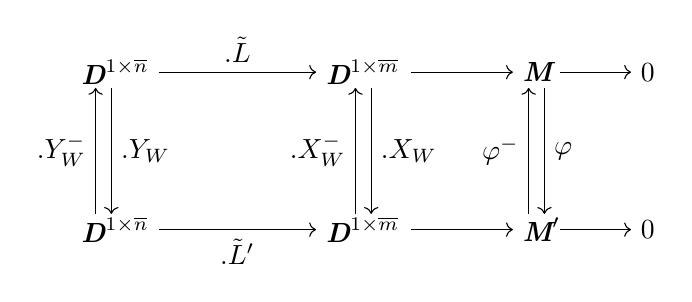
\begin{tikzpicture}
      \coordinate (Rel) at (-4, 0);
      \coordinate (Relsl) at (-4.8, -0.2);
      \coordinate (Relsr) at (-4.6, -0.2);
      \coordinate (Gen) at (-2, 0);
      \coordinate (Genr) at (-0.8, 0);
      \coordinate (Gensl) at (-1.5, -0.2);
      \coordinate (Gensr) at (-1.3, -0.2);
      \coordinate (M) at (0.5, 0);
      \coordinate (Mr) at (1.1, 0);
      \coordinate (Msl) at (0.7, -0.2);
      \coordinate (Msr) at (0.9, -0.2);
      \coordinate (Zero) at (2, 0);

      \coordinate (Relp) at (-4, -2);
      \coordinate (Relpnl) at (-4.8, -1.8);
      \coordinate (Relpnr) at (-4.6, -1.8);
      \coordinate (Genp) at (-2, -2);
      \coordinate (Genpr) at (-0.8, -2);
      \coordinate (Genpnl) at (-1.5, -1.8);
      \coordinate (Genpnr) at (-1.3, -1.8);
      \coordinate (Mp) at (0.5, -2);
      \coordinate (Mpr) at (1.1, -2);
      \coordinate (Mpnl) at (0.7, -1.8);
      \coordinate (Mpnr) at (0.9, -1.8);
      \coordinate (Zerop) at (2, -2);

      \coordinate (R) at (-3, 0);
      \coordinate (Rp) at (-3, -2);

      \coordinate (Qp) at (-4.8, -1);
      \coordinate (Q) at (-4.6, -1);

      \coordinate (Pp) at (-1.5, -1);
      \coordinate (P) at (-1.3, -1);

      \coordinate (phi) at (0.9, -1);
      \coordinate (phip) at (0.7, -1);

      \draw[left] (Rel) node {$\emph{\D}^{1\times\overline{n}}$};
      \draw[right] (Gen) node {$\emph{\D}^{1\times\overline{m}}$};
      \draw[right] (M) node {$\emph{\g{M}}$};
      \draw[right] (Zero) node {$0$};

      \draw[left] (Relp) node {$\emph{\D}^{1\times\overline{n}}$
      };
      \draw[right] (Genp) node {$\emph{\D}^{1\times\overline{m}}$};
      \draw[right] (Mp) node {$\emph{\g{M}}'$};
      \draw[right] (Zerop) node {$0$};

      \draw[above] (R) node {$.\tilde{L}$};
      \draw[below] (Rp) node {$.\tilde{L}'$};
      
      \draw[->] (Rel) -- (Gen);
      \draw[->] (Genr) -- (M);
      \draw[->] (Mr) -- (Zero);
      
      \draw[->] (Relp) -- (Genp);
      \draw[->] (Genpr) -- (Mp);
      \draw[->] (Mpr) -- (Zerop);

      \draw[->] (Mpnl) -- (Msl);
      \draw[->] (Msr) -- (Mpnr);

      \draw[->] (Genpnl) -- (Gensl);
      \draw[->] (Gensr) -- (Genpnr);

      \draw[->] (Relpnl) -- (Relsl);
      \draw[->] (Relsr) -- (Relpnr);

      \draw[left] (Qp) node {$.Y_{W}^-$};
      \draw[right] (Q) node {$.Y_{W}$};

      \draw[left] (Pp) node {$.X_{W}^-$};
      \draw[right] (P) node {$.X_{W}$};

      \draw[left] (phip) node {$\varphi^-$};
      \draw[right] (phi) node {$\varphi$};
    \end{tikzpicture}

  \end{center}
\end{theorem}

\begin{proof}
  We only have to show that the diagram is commutative.

  We show that $Y_W$ and $Y_W^-$ (respectively, $X_W$ and $X_W^-$) are
  inverse to each over in the same manner that we did in the proof of
  Theorem~\ref{thm:reduction_id}.

  Moreover, $Y_W\tilde{L}'=\tilde{L}X_W$ and $Y_W^-\tilde{L}=\tilde{L}'
  X_W^-$ follow from the following commutative diagram:
  \begin{center}
    \begin{equation}\label{equ:main_commutative_diagram_zero_part}
      \begin{tikzcd}
        \D^{1\times\overline{n}}\arrow[d, "\tilde{L}"']\arrow[r, "\iota_r", shift right=-0.5ex] &
        \D^{1\times n}\arrow[d, "L"]\arrow[r, "U_r", shift right=-0.5ex]
        \arrow[l, "\pi_r", shift left=0.5ex] &
        \D^{1\times n}\arrow[d, "L"]\arrow[r, "Y_F", shift right=-0.5ex] 
        \arrow[l, "U_r^-", shift right=-0.5ex] &
        \D^{1\times n}\arrow[d, "L'"]\arrow[r, "\pi'_r", shift right=-0.5ex] 
        \arrow[l, "Y_F^-", shift right=-0.5ex] &
        \D^{1\times\overline{n}}\arrow[d, "\tilde{L}'"]
        \arrow[l, "\iota_r'", shift right=-0.5ex] 
        \\
        \D^{1\times\overline{m}}\arrow[r, "\iota_g", shift right=-0.5ex] &
        \D^{1\times m}\arrow[r, "U_g", shift right=-0.5ex]
        \arrow[l, "\pi_g", shift left=0.5ex] &
        \D^{1\times m}\arrow[r, "X_F", shift right=-0.5ex]
        \arrow[l, "U_g^-", shift right=-0.5ex] &
        \D^{1\times m}\arrow[r, "\pi'_g", shift right=-0.5ex]
        \arrow[l, "X_F^-", shift right=-0.5ex] &
        \D^{1\times\overline{m}}
        \arrow[l, "\iota_g'", shift right=-0.5ex] 
      \end{tikzcd}
    \end{equation}
  \end{center}
  Indeed by computing the matrix products and
  from~\cite{cluzeau2011constructive}, we have the following relations:
  \begin{equation}
    \label{eq:formulas_reduction_id_part}
    \begin{tabular}{l l l l}
      $\iota_rL=\tilde{L}\iota_g,$ & $U_rL=LU_g,$ & $Y_FL'=LX_F$, &
      $\pi_r\tilde{L}=L\pi_g$,\\
      & & \\
      $\iota_r'L'=\tilde{L}'\iota'_g,$ & $Y_F^-L=L'X_F^-,$ & $U_r^-L=LU_g^-$,
      & $\pi_r'\tilde{L}'=L'\pi'_g$.
    \end{tabular}
  \end{equation}
  More details are given in Section~\ref{sec:proofs_reduction_id_part}.
\end{proof}

\section{Annex: proofs}\label{sec:annex}

\subsection{Proof of Formulas~\ref{eq:formulas_reduction_zero_part}}
\label{sec:proofs_reduction_zero_part}

We have to show the following relations

\begin{changemargin}{-1.8cm}{0cm}
  \begin{multicols}{4}
    \begin{equation}\label{equ:eq1_zero_part}
      \iota L=\tilde{L},
    \end{equation}
    
    \begin{equation}\label{equ:eq2_zero_part}
      UL=L,
    \end{equation}
    
    \begin{equation}\label{equ:eq3_zero_part}
      Y_FL'=LX_F,
    \end{equation}
    
    \begin{equation}\label{equ:eq4_zero_part}
      \pi'\tilde{L}'=L',
    \end{equation}
    
    \begin{equation}\label{equ:eq5_zero_part}
      \iota'L'=\tilde{L}',
    \end{equation}
    
    \begin{equation}\label{equ:eq6_zero_part}
      Y_F^-L=L'X_F^-,
    \end{equation}
    
    \begin{equation}\label{equ:eq7_zero_part}
      U^-L=L,
    \end{equation}
    
    \begin{equation}\label{equ:eq8_zero_part}
      \pi\tilde{L}=L.
    \end{equation}
  \end{multicols}
\end{changemargin}

The two relations \eqref{equ:eq3_zero_part} and \eqref{equ:eq6_zero_part}
come from~\cite{cluzeau2011constructive}, \eqref{equ:eq2_zero_part} and
\eqref{equ:eq5_zero_part} are proven by direct computations,
\eqref{equ:eq1_zero_part} and \eqref{equ:eq7_zero_part} are proven by
direct computations using respectively the following two relations:
\[\ell L=0\ \ \text{and}\ \
U^-=\begin{pmatrix}
\id{q+p'} & 0 & 0 & 0\\
0 & \id{p} & 0 & -\g{u}^T\\
0 & 0 & \id{\overline{q'}} & -\g{v}^T\\
0 & 0 & 0 & 1
\end{pmatrix}.\]

In order to prove \eqref{equ:eq4_zero_part}, we first show $\pi'\iota'L'=
L'$: from~\ref{it:split_pip_zero_part} and~\ref{it:ker_pip_zero_part} of
Proposition~\ref{prop:exact_sequences_zero_part}, $\im{\pi'\iota'-\id{n}}
$ is included $\D\ell UY_F$ and using \eqref{equ:eq2_zero_part},
\eqref{equ:eq3_zero_part} and $\ell L=0$, we have $\ell UY_FL'=\ell LUX_F
=0$, which proves the desired relation. Moreover, from
\eqref{equ:eq5_zero_part}, we get $\pi'\iota'L'=\pi'\tilde{L}'$ which,
with $\pi'\iota'L'=L'$, gives \eqref{equ:eq4_zero_part}. We show
\eqref{equ:eq8_zero_part} in the same manner using
\eqref{equ:eq1_zero_part}.

\subsection{Proof of Formulas~\ref{eq:formulas_reduction_id_part}}
\label{sec:proofs_reduction_id_part}

We have to show the following relations

\begin{changemargin}{-1.5cm}{0cm}
  \begin{multicols}{4}
    \begin{equation}\label{equ:eq1_id_part}
      \iota_rL=\tilde{L}\iota_g,
    \end{equation}
    
    \begin{equation}\label{equ:eq2_id_part}
      U_rL=LU_g,
    \end{equation}
    
    \begin{equation}\label{equ:eq3_id_part}
      Y_FL'=LX_F,
    \end{equation}
    
    \begin{equation}\label{equ:eq4_id_part}
      \pi'_r\tilde{L}'=L'\pi'_g,
    \end{equation}
    
    \begin{equation}\label{equ:eq5_id_part}
      \iota'_rL'=\tilde{L}'\iota'_g,
    \end{equation}
    
    \begin{equation}\label{equ:eq6_id_part}
      Y_F^-L=L'X_F^-,
    \end{equation}
    
    \begin{equation}\label{equ:eq7_id_part}
      U_r^-L=LU_g^-, 
    \end{equation}
    
    \begin{equation}\label{equ:eq8_id_part}
      \pi_r\tilde{L}=L\pi_g.
    \end{equation}
  \end{multicols}
\end{changemargin}

The two relations \eqref{equ:eq3_id_part} and \eqref{equ:eq6_id_part}
come from~\cite{cluzeau2011constructive}, \eqref{equ:eq2_id_part} and
\eqref{equ:eq5_id_part} are proven by direct computations,
\eqref{equ:eq7_id_part} is computed by a direct computation using the
inverse formulas for $U_g$ and $U_r$ which are analog to the inverse of
$U$ given in Section~\ref{sec:proofs_reduction_zero_part}.

Let us show \eqref{equ:eq1_id_part}. For that, we decompose $\iota_r$ and
$\iota_g$ in $3$ parts, as follows:
\[
\begin{tabular}{l l l}
  $\iota_r^1:= \begin{pmatrix}
    \id{q+\overline{p'}} & 0 & 0\\
    0 & 0 & \id{p+q'}
  \end{pmatrix},$ &
  $\iota_r^2:= F_r(e^n_{q+p'+p})^T\tilde{\ell}_r\begin{pmatrix}
    \id{q+\overline{p'}} & 0 & 0\\
    0 & 0 & \id{p+q'}
  \end{pmatrix},$ &
  $\iota_r^3:= F_r(e^n_{q+p'+p})^Te^n_{q+p'},$
  \\
  & & \\
  $\iota_g^1:= \begin{pmatrix}
    \id{\overline{m}} & 0
    \end{pmatrix},$ &
  $\iota_g^2:= F_g(e^m_p)^T\ell_g,$ &
  $\iota_g^3:= F_g(e^m_p)^Te^m_{p+p'},$
\end{tabular}
\]
so that we have $\iota_r=\iota_r^1-\iota_r^2+\iota_r^3$ and $\iota_g=
\iota_g^1-\iota_g^2+\iota_g^3$. By compuring the matrix products, we show
that $\iota_r^1L=\tilde{L}\iota_g^1$, that the first $p+\overline{p'}$
columns of $\iota_r^2L$ and $\tilde{L}\iota_g^2$ are both equal to $0$
and their $p+p'$ column are both equal to
\[\begin{pmatrix}
R_{.p}\\
-\left(P'_{ip}+u_iP'_{p'p}\right)_{1\leq i\leq\overline{p'}}\\
0\\
0
\end{pmatrix}.\]
Finally, by computing the matrix products, we show that $\iota_r^3L$ and
$\tilde{L}\iota_g^3$ are respectively equal to
\[\begin{pmatrix}
R_{.p}\\
\left({\id{p'}}_{ip'}-P'P_{ip'}\right)_{1\leq i\leq p'}\\
0\\
0
\end{pmatrix}\begin{pmatrix}
  \g{c}\left(ZR\right)_{p.} & \g{d} & 0
\end{pmatrix}\ \ \text{and}\ \
\begin{pmatrix}
R_{.p}\\
\left({\id{p'}}_{ip'}-P'P_{ip'}\right)_{1\leq i\leq p'}\\
0\\
0
\end{pmatrix}\begin{pmatrix}
  \g{c}\left(\id{p}-PP'\right)_{p.} & \g{d} & 0
\end{pmatrix}\]
so that they are equal from the relation $\id{p}=PP'+ZR$, which proves
\eqref{equ:eq1_id_part}.

Let us show \eqref{equ:eq4_id_part}. By using Relation
\eqref{equ:eq5_id_part}, and~\ref{it:split_pi_id_rel_part} of
Proposition~\ref{prop:exact_sequences_id_rel_part}, we have $\pi'_r
\iota'_rL'\pi'_g=\pi'_r\tilde{L}'$. We proceed as in the proof of
\eqref{equ:eq4_zero_part}: we only have to show that $\im{\pi'_r\iota'_r
  -\id{n}}L'$ is included in $\ker\left(\pi'_g\right)$. We have $\im{
  \pi'_r\iota'_r-\id{n}}\subseteq\D\ell_rU_rY_F$, $\ell_rU_rY_FL'=\ell_r
LU_gX_F$ and $\ell_rL=\ell_g$, so that $\ell_rU_rY_FL'=\ell_gU_gX_F\in
\ker(\pi'_g)$. With the same arguments, we show \eqref{equ:eq4_id_part}.
\bibliography{Biblio}
\end{document}
